\chapter{Le soluzioni}

Una soluzione è una miscela omogenea di due o più sostanze, nella quale si chiama solvente\mkeyword{solvente} la specie in stato liquido che ne determina le proprietà macroscopiche, e soluto\mkeyword{soluto} la specie che vi si scioglie e della quale ci interessano le proprietà chimiche.
La distinzione non è sempre netta, ma di norma il solvente è presente in largo eccesso ed è quello che impone lo stato di aggregazione alla miscela.\\

Le interazioni che si stabiliscono in soluzione si dividono in tre categorie.

Le interazioni aspecifiche\mkeyword{interazioni aspecifiche} sono di natura fisica e prevalentemente elettrostatica, non dipendono dall'identità chimica delle molecole coinvolte e agiscono sempre.

Le interazioni specifiche\mkeyword{interazioni specifiche} hanno invece carattere chimico e richiedono che le molecole possiedano gruppi funzionali particolari, come nel caso del legame a idrogeno.

Le interazioni chimiche vere e proprie, infine, comportano la formazione di legami fra soluto e solvente e portano a specie nuove.\\

Dal punto di vista strutturale conviene distinguere due regioni del solvente.

\begin{figure}[htbp]
    \centering
    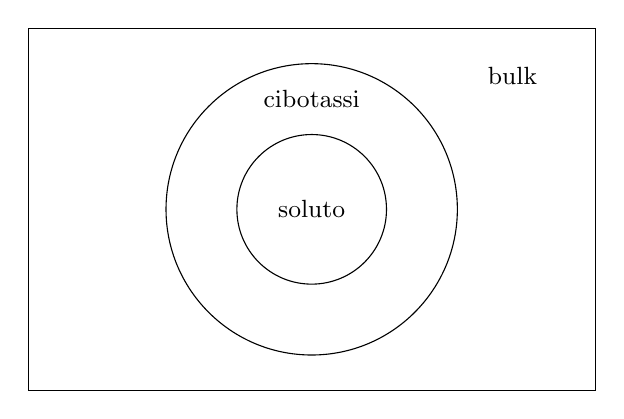
\begin{tikzpicture}
        % --- macro riutilizzabili -----------------------------------------
        \def\rsoluto{0.95}
        \def\rcluster{1.85}
        \def\etichetta#1#2{\node[font=\small] at #1 {#2};}
        % --- cornice del solvente -----------------------------------------
        \draw (-3.60,-2.30) rectangle (3.60,2.30);
        % --- regioni ------------------------------------------------------
        \draw (0,0) circle (\rcluster);
        \draw (0,0) circle (\rsoluto);
        % --- etichette ----------------------------------------------------
        \etichetta{(0,0)}{soluto}
        \etichetta{(0,1.40)}{cibotassi}
        \etichetta{(2.55,1.70)}{bulk}
    \end{tikzpicture}
    \caption{Struttura di una soluzione attorno a una molecola di soluto.}
\end{figure}


Le molecole di solvente immediatamente vicine al soluto ne risentono direttamente e si dispongono in modo ordinato attorno a esso, formando quello che si chiama cibotassi\mkeyword{cibotassi}. 

Il resto del solvente, detto bulk\mkeyword{bulk}, risente della presenza del soluto solo attraverso interazioni aspecifiche e si comporta essenzialmente come solvente puro.

\newpage

\section{Il ciclo di solvatazione}

Per capire che cosa determini la solubilità conviene scomporre il processo in passi ideali.

Si immagina di estrarre una molecola di soluto dal suo stato condensato portandola in fase gassosa; si crea poi nel solvente una cavità capace di ospitarla; infine si inserisce la molecola isolata nella cavità, dove stabilisce interazioni con il solvente.
La molecola così sistemata si dice solvatata\mkeyword{solvatazione}, e il bilancio complessivo è

\begin{equation}
    \Delta G_{sol} = \underbrace{\Delta G_{soluto}}_{>0} + \underbrace{\Delta G_{cavit\grave{a}}}_{>0} + \underbrace{\Delta G_{soluto-solvente}}_{<0} .
    \label{eq:ciclo_solvatazione}
\end{equation}

Il processo è spontaneo, e dunque la sostanza è solubile, quando la somma risulta negativa: i primi due termini sono costi da pagare, il terzo è il guadagno che li deve compensare.
Il ciclo è naturalmente un artificio, poiché nessuno dei tre passi avviene realmente in isolamento, ma poiché $G$ è una funzione di stato il bilancio complessivo non dipende dal cammino scelto per calcolarlo.

\subsection{Le interazioni all'interno del soluto}

Il primo termine della \eqref{eq:ciclo_solvatazione} è il costo di smontare il soluto, e dipende da quali forze lo tengono insieme.

\begin{table}[htbp]
    \centering
    \begin{tabular}{lll}
        \toprule
        Tipo di soluto & Interazione dominante & Costo \\
        \midrule
        solidi e liquidi ionici     & energia reticolare, elettrostatica & altissimo \\
        solidi molecolari altofondenti & dipolo-dipolo e legame a idrogeno & alto \\
        solidi molecolari bassofondenti & dispersione e repulsione & basso \\
        solidi e liquidi metallici  & condivisione degli elettroni di valenza & altissimo \\
        \bottomrule
    \end{tabular}
    \caption{Interazioni interne al soluto e costo relativo della loro rottura.}
    \label{tab:interazioni_soluto}
\end{table}

Dall'elenco mancano volutamente i solidi covalenti reticolari, per la ragione che non si sciolgono in nulla: sciogliere il diamante richiederebbe di rompere una rete continua di legami covalenti, e nessuna interazione con il solvente può ripagare un costo simile.

\subsection{Le interazioni fra soluto e solvente}

Il secondo e il terzo termine della \eqref{eq:ciclo_solvatazione} si scompongono a loro volta in cinque contributi, dei quali due destabilizzanti, con $\Delta G > 0$, e tre stabilizzanti, con $\Delta G < 0$.\\

La cavitazione\mkeyword{cavitazione} è il costo di aprire nel bulk del solvente uno spazio capace di contenere la molecola di soluto, e comporta la rottura di interazioni solvente-solvente.
È tanto maggiore quanto più il solvente è coeso: in prima approssimazione il costo è proporzionale alla superficie della cavità creata e alla tensione superficiale del solvente.
Dipende quindi dalle dimensioni e dalla forma del soluto, e non dalla sua natura chimica.\\

\newpage

L'interazione elettrostatica\mkeyword{interazione elettrostatica} è il contributo dovuto alla distribuzione di carica del soluto, che genera un campo nel solvente e vi induce una polarizzazione: le molecole di solvente si orientano in modo da minimizzare l'energia.
È l'unico contributo a lungo raggio, e dipende dalla costante dielettrica del solvente e dalla carica del soluto, risultando dominante per gli ioni e per le molecole molto polari.\\

La dispersione\mkeyword{dispersione} è l'interazione fra le fluttuazioni istantanee della densità di carica del soluto e quelle del solvente, cioè la forza di London già studiata: decade come $r^{-6}$, è a corto raggio e dipende dalle dimensioni molecolari, ed è sempre stabilizzante.\\

La repulsione\mkeyword{repulsione} nasce dalla sovrapposizione delle nubi elettroniche di soluto e solvente e dal principio di esclusione di Pauli: decade come $r^{-12}$, è una forza di contatto ed è sempre destabilizzante.
Insieme alla dispersione costituisce i due rami del potenziale di Lennard-Jones applicato alla coppia soluto-solvente, e diventa determinante soltanto in condizioni estreme di pressione, dove ha rilevanza geochimica.\\

La variazione geometrica\mkeyword{variazione geometrica}, infine, riguarda il soluto stesso, che una volta immerso nel solvente adotta una geometria diversa da quella che aveva isolato.
I solventi polari tendono ad accentuare il dipolo del soluto, i solventi apolari a ridurlo, ed essendo la deformazione adottata soltanto quando conviene, il bilancio di questo contributo è stabilizzante.

\subsection{Il bilancio complessivo}

Sommando i cinque contributi si osserva una regolarità.

Le interazioni non specifiche, cioè cavitazione, dispersione e repulsione, danno complessivamente un contributo sfavorevole, e dipendono dalle dimensioni della molecola di soluto e da quanto il solvente è strutturato.
Perché la sostanza sia solubile occorre dunque che i contributi elettrostatico e geometrico, i quali dipendono dalla struttura chimica e in particolare dalla presenza di cariche nette o di gruppi polari, siano abbastanza negativi da compensarli.\\

Questa è la formulazione quantitativa del principio empirico secondo cui il simile scioglie il simile.

Un solvente polare come l'acqua scioglie bene sostanze ioniche e polari, perché offre un termine elettrostatico grande, mentre non scioglie sostanze apolari, per le quali quel termine è nullo e resta soltanto un costo di cavitazione elevato.

Un solvente apolare, al contrario, ha un costo di cavitazione modesto, e quindi la sola dispersione basta a compensarlo: i soluti apolari vi si sciolgono senza bisogno di alcun contributo elettrostatico.

\newpage

\section{Solubilità e prodotto di solubilità}

Per ogni coppia soluto-solvente esiste una quantità massima di soluto che può essere portata in soluzione, detta solubilità\mkeyword{solubilità} e indicata con $s$, misurata in $g/L$ oppure, più comodamente per i calcoli, in $mol/L$.
Una soluzione che abbia raggiunto tale valore si dice satura\mkeyword{soluzione satura}, e il soluto eventualmente aggiunto in eccesso non si scioglie ma resta come corpo di fondo.\\

In presenza di corpo di fondo il sistema non è inerte ma si trova all'equilibrio dinamico fra la fase solida e le specie disciolte.

Per un generico sale di formula $\mathrm{M}_x\mathrm{A}_y$ tale equilibrio si scrive

\begin{equation}
    \mathrm{M}_x\mathrm{A}_{y\,(s)} \rightleftharpoons x\,\mathrm{M}^{y+}_{(aq)} + y\,\mathrm{A}^{x-}_{(aq)} ,
    \label{eq:equilibrio_sale}
\end{equation}

e la sua costante di equilibrio non contiene il reagente, poiché la concentrazione di una fase condensata pura non dipende dalla quantità presente ma soltanto dalla densità della sostanza, ed è quindi una costante che viene inglobata nella costante di equilibrio stessa.

Ciò che resta è il solo prodotto delle concentrazioni ioniche, detto per questa ragione prodotto di solubilità\mkeyword{prodotto di solubilità}:

\begin{equation}
    K_{ps} = [\mathrm{M}^{y+}]^x\,[\mathrm{A}^{x-}]^y .
    \label{eq:kps}
\end{equation}

Si tratta di una costante di equilibrio a tutti gli effetti, e come tale dipende dalla sola temperatura; va però ricordato che la \eqref{eq:kps} descrive esclusivamente soluzioni sature, cioè in presenza di corpo di fondo, poiché soltanto in tali condizioni il sistema è all'equilibrio.\\

Il legame fra $K_{ps}$ e la solubilità si ottiene con un bilancio di massa.
Se si sciolgono $s$ moli di sale per litro, ciascuna di esse libera $x$ ioni $\mathrm{M}^{y+}$ e $y$ ioni $\mathrm{A}^{x-}$, cosicché all'equilibrio si ha $[\mathrm{M}^{y+}] = xs$ e $[\mathrm{A}^{x-}] = ys$.

Sostituendo nella \eqref{eq:kps} si ricava

\begin{equation}
    K_{ps} = (xs)^x (ys)^y = x^x y^y\, s^{x+y}
    \qquad\Longrightarrow\qquad
    s = \left(\frac{K_{ps}}{x^x y^y}\right)^{1/(x+y)} .
    \label{eq:kps_generale}
\end{equation}

Si osservi che i coefficienti stechiometrici intervengono due volte e per ragioni distinte, come fattori moltiplicativi nelle concentrazioni, per via del bilancio di massa, e come esponenti nella costante, per via della stechiometria dell'equilibrio.
